% =====================================================================
%  Unit 7 -- Applications
%  (this file is assembled from src/ch07/*.tex by build_chapter.py)
% =====================================================================
\chapter{Applications}\label{ch:applications}

In 2015 Netflix\index{Netflix Prize} estimated that about 80\% of the hours streamed on its service were influenced by its
recommendations, and that personalisation and recommendations saved it more than one billion dollars a year, mostly by keeping
subscribers who would otherwise cancel \citep{gomezuribe2015netflix}. This example shows how a model can affect the
results of a company directly, and how evaluation, deployment\index{deployment} and monitoring\index{monitoring} come together in practice.

The previous units built, evaluated, combined, deployed and monitored models in general. This last unit
looks at two families of applications in which machine learning creates direct business value, and at a
tool for putting models in the hands of their users. \emph{Recommender systems\index{recommender system|textbf}} suggest products, films,
songs or people to each user according to their preferences, and they drive a large share of what is
bought, watched and read online. \emph{Customer relationship management\index{customer relationship management (CRM)|textbf}} (CRM) uses data about customers to
decide whom to contact, with what and when; we will see how to design a marketing campaign\index{mailing campaign} with a
probabilistic classifier and cost information, and why the customers most likely to buy are not
necessarily the ones worth contacting. Finally, \emph{Shiny\index{Shiny|textbf}} turns a model into an interactive web
application with a few lines of code. Many ideas from earlier units reappear: ranking metrics and costs
(\cref{ch:evaluation}), causality\index{causality} (\cref{sec:causality}), experiments and bandits\index{multi-armed bandit}
(\cref{sec:abtesting,sec:bandits}) and web applications (\cref{sec:webapps}). The unit closes by following both applications through the whole life cycle, from evaluation to
updating.

\begin{objectives}
After studying this unit you should be able to:
\begin{itemize}
  \item describe the main approaches to recommendation (collaborative filtering\index{collaborative filtering}, content-based\index{content-based filtering} filtering and
        hybrids) and their strengths and weaknesses;
  \item compute user and item similarities and the recommendations of neighbourhood methods by hand, and
        explain matrix factorisation\index{matrix factorisation};
  \item evaluate recommenders for rating prediction and for top-$N$ recommendation, including measures beyond
        accuracy\index{accuracy} such as coverage\index{coverage} and novelty\index{novelty};
  \item design a targeted mailing campaign with a pilot sample, a probabilistic classifier, cumulative response
        curves and profit curves\index{profit curve};
  \item explain uplift\index{uplift modelling} modelling and why it targets different customers than a response model;
\item design a churn model with a temporal protocol, and rank customers by the value that a retention
offer saves;
  \item build an interactive application with Shiny, using reactive\index{reactive programming} expressions to avoid unnecessary computation,
        and test it;
\item plan the evaluation, deployment, monitoring and updating of a recommender or a customer campaign.
\end{itemize}
\end{objectives}

% =====================================================================
\section{Recommender systems}\label{sec:recsys}

Imagine that you want to buy a new phone. You can compare technical features, or you can ask friends and
other people who bought one. Recommender systems\index{recommender system} automate both strategies, and they are widely used: films
and series on streaming platforms, songs and podcasts, products in online shops, hotels and restaurants,
videos, apps, news, jobs and even partners on dating applications. Their input is usually a set of
interactions between users and items, either \emph{explicit} (ratings, likes) or \emph{implicit} (purchases,
clicks, viewing time), which can be arranged as a large and very sparse \emph{user--item matrix}: most users
have interacted with a tiny fraction of the items. The main approaches (\cref{fig:rectaxonomy}) are
\citep{aggarwal2016recommender,ricci2022recommender}:
\begin{itemize}
  \item \emph{collaborative filtering\index{collaborative filtering|textbf}}, which learns from the user--item interactions alone, using
        similarities between users or between items, or models of their latent preferences;
  \item \emph{content-based\index{content-based filtering|textbf} filtering}, which recommends items similar, in their attributes or descriptions, to
        those the user liked;
  \item \emph{hybrid} systems, which combine both, as most large-scale recommenders do.
\end{itemize}

\begin{figure}[htbp]
\centering
\begin{tikzpicture}[font=\scriptsize\sffamily,
  root/.style={draw=edmnavy,fill=edmnavy!12,rounded corners=2pt,minimum height=7mm,align=center,font=\scriptsize\sffamily\bfseries},
  mid/.style={draw=edmnavy,fill=edmnavy!5,rounded corners=2pt,minimum height=7mm,minimum width=27mm,align=center},
  leaf/.style={draw=edmnavy!60,rounded corners=2pt,minimum height=6mm,minimum width=22mm,align=center,font=\tiny\sffamily},
  arr/.style={-{Stealth[length=1.5mm]},edmnavy!80}]
  \node[root] (r) at (0,0) {recommender systems};
  \node[mid] (cf) at (-4.2,-1.2) {collaborative filtering\\(interactions only)};
  \node[mid] (cb) at (0,-1.2) {content-based\\(item descriptions)};
  \node[mid] (hy) at (4.2,-1.2) {hybrid\\(both)};
  \node[leaf] (mb) at (-5.6,-2.5) {memory-based:\\user- or item-based\\neighbours};
  \node[leaf] (mo) at (-2.8,-2.5) {model-based:\\matrix factorisation,\\neural models};
  \node[leaf] (c1) at (0,-2.5) {attributes, text\\(TF-IDF), images};
  \node[leaf] (h1) at (4.2,-2.5) {weighted, switching,\\feature combination};
  \foreach \a/\b in {r/cf,r/cb,r/hy,cf/mb,cf/mo,cb/c1,hy/h1} \draw[arr] (\a) -- (\b);
\end{tikzpicture}
\caption{The main families of recommender systems.}
\label{fig:rectaxonomy}
\end{figure}

% ---------------------------------------------------------------------
\section{Collaborative filtering}\label{sec:cf}

Collaborative filtering\index{collaborative filtering} rests on a simple intuition: users who agreed in the past tend to agree in the future,
so the opinions of users with tastes similar to mine are good predictors of what I will like
\citep{resnick1994grouplens}. Two things must be defined: a measure of the similarity\index{similarity measure} between users, and a way
of combining the opinions of similar users into recommendations, weighted by their similarity
\citep{segaran2007programming}.

\subsection{Similarity between users}

Each user is a row of the rating matrix, a vector with many missing values, and two users can be compared on the
items that both have rated. \Cref{lst:ratingstoy} defines a small, made-up matrix of seven users and six films, and
two classic measures:
\begin{itemize}
  \item a similarity\index{similarity measure} derived from the \emph{Euclidean\index{Euclidean distance|textbf} distance} between the two vectors of common ratings,
        $\mathrm{sim}(u,v)=1/(1+d(u,v))$, which is 1 for identical ratings and decreases with the distance. Users
        become points in a space with one axis per item (\cref{fig:similarity}b). Because it adds up the
        differences, it also falls with the number of common items (a difference of one star gives 0.5 on one
        film and 0.24 on ten), so users with different overlaps are not directly comparable;
  \item the \emph{Pearson\index{Pearson correlation|textbf} correlation} of the common ratings, which measures their linear association after
        centring the ratings of each user, regardless of how generous each one is: a user who always gives one star more than another
        has a correlation of 1 with them (\cref{fig:similarity}a). Other choices are the cosine\index{cosine similarity} of the rating
        vectors, rank correlations (Spearman\index{Spearman correlation}, Kendall) and, for binary interactions, the Jaccard index.
\end{itemize}

\begin{pylisting}[label={lst:ratingstoy}]{A small rating matrix and two similarity measures (file \texttt{ratings\_toy.py})}
"""A small, made-up rating matrix (1-5 stars) and two similarity measures (Unit 7)."""
import numpy as np

nan = np.nan
FILMS = ["Space Saga", "Paris Love", "Heist Night", "Silent Forest", "Laugh Club",
         "Deep Ocean"]
USERS = ["Ana", "Ben", "Carla", "David", "Elena", "Fran", "Ivo"]
R = np.array([[4.5, 2.0, 4.0, 3.0, 2.5, 4.0],      # Ana
              [5.0, 1.5, 4.5, nan, 2.0, 3.5],      # Ben
              [2.0, 4.5, 2.5, 4.0, 4.5, nan],      # Carla
              [nan, 4.0, 2.0, 3.5, 5.0, 2.5],      # David
              [3.5, 3.0, nan, 4.5, 3.0, 4.0],      # Elena
              [4.0, nan, 3.5, 2.0, nan, 4.5],      # Fran
              [4.0, nan, nan, nan, 2.0, 4.5]])     # Ivo, who wants recommendations

def euclidean_similarity(a, b):
    """1 / (1 + Euclidean distance) over the items rated by both."""
    both = ~np.isnan(a) & ~np.isnan(b)
    return 1 / (1 + np.sqrt(np.sum((a[both] - b[both]) ** 2))) if both.any() else 0.0

def pearson(a, b):
    """Pearson correlation over the items rated by both (0 if undefined)."""
    both = ~np.isnan(a) & ~np.isnan(b)
    if both.sum() < 2 or a[both].std() == 0 or b[both].std() == 0:
        return 0.0
    return float(np.corrcoef(a[both], b[both])[0, 1])
\end{pylisting}

\begin{figure}[htbp]
\centering
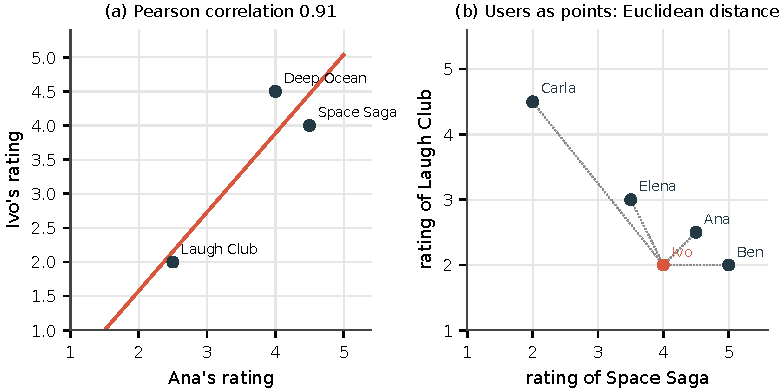
\includegraphics[width=\textwidth]{ch07/similarity}
\caption{(a) Ana's and Ivo's ratings of the three films they have both seen, and the regression line behind their
Pearson correlation. (b) Users as points in the plane of two of the films; the dotted lines are the Euclidean
distances to Ivo in this plane only, not over all the films each pair has in common.}
\label{fig:similarity}
\end{figure}

\subsection{From similar users to recommendations}

To recommend films to Ivo, we could take the most similar user and suggest the film they rated highest among those Ivo
has not seen. This is too local a strategy: it relies on the opinion of a single person and ignores every film that
person has not rated. It is better to combine the ratings of several users, using their similarities as weights. For
an item $i$ that user $u$ has not rated, the predicted rating is the weighted average of the ratings of the users $v$ who
rated it,
\begin{equation}\label{eq:usercf}
  \hat r_{ui}=\frac{\sum_{v}\mathrm{sim}(u,v)\,r_{vi}}{\sum_{v}\mathrm{sim}(u,v)},
\end{equation}
where the sums run over the users with a positive similarity\index{similarity measure} who rated $i$ (often only the $k$ most similar ones).
Dividing by the sum of the similarities of the users who rated \emph{that} item matters: otherwise films seen by many
people would get high totals just for being popular. A refinement predicts deviations from each user's mean rating,
$\hat r_{ui}=\bar r_u+\sum_v\mathrm{sim}(u,v)(r_{vi}-\bar r_v)/\sum_v|\mathrm{sim}(u,v)|$, which corrects for users who
rate generously or harshly.

\begin{pylisting}[label={lst:usercf}]{User-based collaborative filtering with Pearson similarities}
import numpy as np
from ratings_toy import FILMS, R, USERS, euclidean_similarity, pearson

me = USERS.index("Ivo")
print("similarity of Ivo to   " + "  ".join(f"{u:>6s}" for u in USERS[:-1]))
for name, sim in [("Euclidean-based", euclidean_similarity), ("Pearson", pearson)]:
    print(f"{name:22s}" + "  ".join(f"{sim(R[me], R[v]):6.2f}" for v in range(me)))

def recommend(user, sim=pearson):
    """Weighted average of the others' ratings, with positive similarities as weights."""
    rows = []
    for i, film in enumerate(FILMS):
        if not np.isnan(R[user, i]):
            continue                                   # already seen
        total = sim_sum = 0.0
        for v in range(len(USERS)):
            s = sim(R[user], R[v]) if v != user else 0.0
            if s > 0 and not np.isnan(R[v, i]):
                total += s * R[v, i]
                sim_sum += s
        rows.append((film, total, sim_sum, total / sim_sum if sim_sum else np.nan))
    return sorted(rows, key=lambda r: -r[3])

print("film            total   sim. sum   predicted rating")
for film, total, sim_sum, score in recommend(me):
    print(f"{film:14s} {total:6.2f}   {sim_sum:6.2f}       {score:.2f}")
\end{pylisting}
\begin{pyoutput}
similarity of Ivo to      Ana     Ben   Carla   David   Elena    Fran
Euclidean-based         0.54    0.41    0.24    0.22    0.45    1.00
Pearson                 0.91    0.76   -1.00   -1.00    0.94    1.00
film            total   sim. sum   predicted rating
Heist Night     10.53     2.66       3.95
Silent Forest    8.98     2.85       3.15
Paris Love       5.78     2.61       2.22
\end{pyoutput}

\Cref{lst:usercf} computes both similarities between Ivo and the other users and builds the table of
\cref{eq:usercf}: for each unseen film, the total of the similarity-weighted ratings, the sum of the similarities of the
users who rated it, and their ratio. \emph{Heist Night} is the clear recommendation (3.95), and \emph{Paris Love}, loved
by the users whose tastes are opposite to Ivo's, is the clear non-recommendation (2.22). The table also shows a weakness of
the Pearson\index{Pearson correlation} correlation: with only two films in common, it is always $+1$ or $-1$ when both users rated the two films differently
(Carla, David and Fran), whatever the ratings, because two points always lie on a line; it is undefined,
and taken as 0 by the code, when a user gave both films the same rating. In practice, similarities computed on few common items are shrunk towards
zero (\emph{significance weighting}), or a minimum number of common items is required.

\subsection{Item-based collaborative filtering}\label{sec:itemcf}

User-based\index{collaborative filtering!user-based} filtering does not scale well: with millions of users, finding the neighbours of each user at request time is
expensive, and when the catalogue is large two users rarely have enough items in common to be compared reliably. Item-based filtering compares \emph{items}: two films are similar if the users who rated both rated them
alike, which is the same computation applied to the columns of the matrix. To recommend items to a user, we
look for items similar to those the user rated, weighted by their similarity\index{similarity measure} and by the user's ratings
\citep{sarwar2001item}. Similarities between items are more stable than similarities between users, because each item has
many ratings and its audience changes slowly, so the item--item matrix can be precomputed offline and updated
infrequently, which makes recommendation fast. This is how Amazon's recommendations worked at scale
\citep{linden2003amazon}.

A note on terminology: item-based\index{collaborative filtering!item-based} filtering, which some texts call ``content-based\index{content-based filtering}'' because it relies on similarities
between items, is still \emph{collaborative}: the similarities come from the users' ratings. They do not use the attributes of the items. Content-based filtering in the strict sense, which uses the descriptions of the items, is the subject of
\cref{sec:contentbased}.

\begin{pylisting}[label={lst:itemcf}]{Item-based collaborative filtering, and recommending users to an item}
import numpy as np
from ratings_toy import FILMS, R, USERS, pearson

# Item-based: precompute item-item similarities once (the columns of the matrix)
n = len(FILMS)
S = np.array([[pearson(R[:, i], R[:, j]) if i != j else -np.inf for j in range(n)]
              for i in range(n)])
print("films most similar to 'Space Saga':",
      ", ".join(f"{FILMS[j]} ({S[0, j]:+.2f})" for j in np.argsort(-S[0])[:2]))

def recommend_items(user):
    seen = ~np.isnan(R[user])
    scores = {}
    for i in np.flatnonzero(~seen):
        w = np.maximum(S[i, seen], 0)                  # similar items the user has rated
        if w.sum() > 0:
            scores[FILMS[i]] = float(w @ R[user, seen] / w.sum())
    return sorted(scores.items(), key=lambda kv: -kv[1])

print("item-based recommendations for Ivo:",
      ", ".join(f"{f} {s:.2f}" for f, s in recommend_items(USERS.index("Ivo"))))

# Recommending users to an item: who has not seen it, and would rate it highest?
film = FILMS.index("Silent Forest")
pred = {}
for u in np.flatnonzero(np.isnan(R[:, film])):
    w = np.array([max(pearson(R[u], R[v]), 0) if v != u and not np.isnan(R[v, film])
                  else 0.0 for v in range(len(USERS))])
    if w.sum() > 0:                                    # else: no evidence, no ranking
        pred[USERS[u]] = float(w @ np.nan_to_num(R[:, film]) / w.sum())
print("who should be told about 'Silent Forest':",
      ", ".join(f"{u} {s:.2f}" for u, s in sorted(pred.items(), key=lambda kv: -kv[1])))
\end{pylisting}
\begin{pyoutput}
films most similar to 'Space Saga': Heist Night (+0.98), Silent Forest (-0.56)
item-based recommendations for Ivo: Heist Night 4.20, Paris Love 2.00, Silent Forest 2.00
who should be told about 'Silent Forest': Ben 3.61, Ivo 3.15
\end{pyoutput}

In \cref{lst:itemcf}, the film most similar to \emph{Space Saga} is \emph{Heist Night} (+0.98), and the item-based
recommendations for Ivo again put \emph{Heist Night} first (4.20). The same machinery can be turned around to
\emph{recommend users to items}, for instance to find the customers for a product that must be promoted. If the item already has enough ratings, the matrix is transposed, or the predicted ratings of the users who have not seen the item are ranked. A brand-new film with no ratings needs the content-based methods of \cref{sec:contentbased}. Ben (3.61) and Ivo (3.15) are the
users who should be told about \emph{Silent Forest}.

The choice between the two depends on the setting \citep{segaran2007programming}. Item-based filtering is faster at
recommendation time but needs to store and update the item--item similarities, and it gives more robust results on sparse
data sets, where similar users are hard to find (some services ask new users to rate a few items to bootstrap their
profile). User-based filtering is often better in small and dynamic settings, and in social networks the information about
friends can be exploited directly.

% ---------------------------------------------------------------------
\section{Matrix factorisation and the Netflix Prize\extsec}\label{sec:mf}

Neighbourhood methods are \emph{memory-based}: they keep the data and compute similarities. \emph{Model-based} methods
learn a compact model of the preferences instead. A widely used one is \emph{matrix factorisation\index{matrix factorisation|textbf}}. It represents
every user $u$ and every item $i$ by vectors $p_u$ and $q_i$ of $k$ \emph{latent factors}, numbers learned from the ratings that may capture, for instance, how much a film is a comedy and how much a user likes comedies (the factors have no names). It predicts a rating from the dot
product of the two vectors plus biases \citep{koren2009matrix}:
\begin{equation}\label{eq:mf}
  \hat r_{ui}=\mu+b_u+b_i+p_u^\top q_i,\qquad
  \min_{b,p,q}\sum_{(u,i)\ \text{observed}}\Bigl[\bigl(r_{ui}-\hat r_{ui}\bigr)^2
  +\lambda\bigl(b_u^2+b_i^2+\|p_u\|^2+\|q_i\|^2\bigr)\Bigr],
\end{equation}
where $\mu$ is the global mean, $b_u$ and $b_i$ capture generous users and popular items, and the sum runs only over the
observed ratings; each parameter is penalised once for every rating in which it takes part, as in the
stochastic gradient updates of the listing. The parameters are fitted by stochastic gradient descent or by alternating least squares, and the
regularisation $\lambda$ prevents the factors of users and items with few ratings from overfitting\index{overfitting}.

Matrix factorisation came to prominence with the \emph{Netflix\index{Netflix Prize|textbf} Prize}, a competition run by Netflix from 2006 to 2009
\citep{bennett2007netflix}. Netflix released 100,480,507 ratings (from 1 to 5 stars, with their dates) given by 480,189
users to 17,770 films, and offered one million dollars to the first team that improved the error of its own recommender\index{recommender system}
by 10\% in RMSE\index{root mean squared error (RMSE)}. The prize was won in 2009 by a team that blended hundreds of models, of which factorisation and neighbourhood
models were the core. The competition also left a lesson about privacy: although the data had been anonymised,
\citet{narayanan2008robust} showed that users could be re-identified by matching their ratings with public reviews on the Internet Movie
Database, and a planned second competition was cancelled. Ratings reveal much about people,
and the precautions of \cref{sec:fairness} apply.

\begin{pylisting}[label={lst:recmodels}]{Synthetic ratings, biases, neighbours and matrix factorisation (file \texttt{recsys\_models.py})}
"""Synthetic ratings and three recommenders: biases, neighbours, matrix factorisation."""
import numpy as np

def make_ratings(n_users=600, n_items=400, k=5, seed=0, return_truth=False):
    """Ratings from latent tastes. Users rate popular items and items they like more
    often: the missing ratings are not missing at random."""
    rng = np.random.default_rng(seed)
    P, Q = rng.normal(0, 0.8, (n_users, k)), rng.normal(0, 0.8, (n_items, k))
    bu, bi = rng.normal(0, 0.4, n_users), rng.normal(0, 0.5, n_items)
    true = 3.3 + bu[:, None] + bi[None, :] + P @ Q.T
    pop = np.exp(1.2 * bi + rng.normal(0, 1.0, n_items))
    R_train = np.full((n_users, n_items), np.nan)
    test = []
    for u in range(n_users):
        w = pop * np.exp(0.5 * (P[u] @ Q.T))           # popularity and personal taste
        items = rng.choice(n_items, 8 + rng.poisson(15), replace=False, p=w / w.sum())
        r = np.clip(np.round(true[u, items] + rng.normal(0, 0.5, len(items))), 1, 5)
        order = rng.permutation(len(items))            # a random split of the history
        items, r = items[order], r[order]
        cut = max(1, len(items) // 5)                  # about 20% for testing
        R_train[u, items[cut:]] = r[cut:]
        test += [(u, i, x) for i, x in zip(items[:cut], r[:cut])]
    return (R_train, np.array(test), true) if return_truth else (R_train, np.array(test))

def fit_biases(R, reg=5.0, iterations=10):
    obs, Rz, mu = ~np.isnan(R), np.nan_to_num(R), np.nanmean(R)
    bu, bi = np.zeros(R.shape[0]), np.zeros(R.shape[1])
    for _ in range(iterations):                        # alternating regularised means
        bi = ((Rz - mu - bu[:, None]) * obs).sum(0) / (reg + obs.sum(0))
        bu = ((Rz - mu - bi[None, :]) * obs).sum(1) / (reg + obs.sum(1))
    return lambda u, i: np.clip(mu + bu[u] + bi[i], 1, 5)

def knn(R, by="item", k=30):
    """Neighbourhood model on mean-centred ratings (cosine of centred vectors)."""
    M = R.T if by == "item" else R                     # rows: the entities compared
    counts = np.sum(~np.isnan(M), axis=1)
    mu = np.where(counts > 0, np.nansum(M, axis=1) / np.maximum(counts, 1), np.nanmean(M))
    C = np.nan_to_num(M - mu[:, None])
    norm = np.linalg.norm(C, axis=1) + 1e-9
    S = C @ C.T / np.outer(norm, norm)
    np.fill_diagonal(S, 0)

    def predict(u, i):
        a, b = (i, u) if by == "item" else (u, i)      # predict entity a for column b
        cand = np.flatnonzero(~np.isnan(M[:, b]))
        top = cand[np.argsort(-S[a, cand])[:k]]
        w = S[a, top]
        if np.abs(w).sum() < 1e-9:
            return mu[a]
        return float(np.clip(mu[a] + w @ C[top, b] / np.abs(w).sum(), 1, 5))
    return predict

def fit_mf(R, k=10, lr=0.01, reg=0.05, epochs=40, seed=0):
    """Matrix factorisation with biases, trained by stochastic gradient descent."""
    rng = np.random.default_rng(seed)
    users, items = np.nonzero(~np.isnan(R))
    r, mu = R[users, items], np.nanmean(R)
    bu, bi = np.zeros(R.shape[0]), np.zeros(R.shape[1])
    P, Q = rng.normal(0, 0.1, (R.shape[0], k)), rng.normal(0, 0.1, (R.shape[1], k))
    for _ in range(epochs):
        for j in rng.permutation(len(r)):
            u, i = users[j], items[j]
            e = r[j] - (mu + bu[u] + bi[i] + P[u] @ Q[i])
            bu[u] += lr * (e - reg * bu[u])
            bi[i] += lr * (e - reg * bi[i])
            pu = P[u].copy()
            P[u] += lr * (e * Q[i] - reg * P[u])
            Q[i] += lr * (e * pu - reg * Q[i])
    return lambda u, i: np.clip(mu + bu[u] + bi[i] + np.sum(P[u] * Q[i], axis=-1), 1, 5)
\end{pylisting}

\begin{pylisting}[label={lst:ratingpred}]{Predicting held-out ratings with five methods}
import numpy as np
from recsys_models import fit_biases, fit_mf, knn, make_ratings

R, test = make_ratings()
u, i, r = test[:, 0].astype(int), test[:, 1].astype(int), test[:, 2]
print(f"{R.shape[0]} users, {R.shape[1]} items, {np.sum(~np.isnan(R))} training ratings "
      f"({np.mean(~np.isnan(R)):.1%} of the matrix), {len(r)} test ratings")
rmse = lambda pred: np.sqrt(np.mean((np.asarray(pred) - r) ** 2))
models = {"global mean": lambda u, i: np.full(len(u), np.nanmean(R)),
          "user and item biases": fit_biases(R),
          "user-based neighbours": np.vectorize(knn(R, by="user")),
          "item-based neighbours": np.vectorize(knn(R, by="item")),
          "matrix factorisation": fit_mf(R)}
results = {name: rmse(model(u, i)) for name, model in models.items()}
for name, value in results.items():
    print(f"{name:22s} RMSE {value:.3f}")
\end{pylisting}
\begin{pyoutput}
600 users, 400 items, 11192 training ratings (4.7% of the matrix), 2486 test ratings
global mean            RMSE 1.064
user and item biases   RMSE 0.983
user-based neighbours  RMSE 0.962
item-based neighbours  RMSE 0.946
matrix factorisation   RMSE 0.952
\end{pyoutput}

\Cref{lst:recmodels} generates ratings for 600 users and 400 items from five latent tastes, with a realistic feature that
matters later: users rate popular items, and items they expect to like, more often. \Cref{lst:ratingpred} holds out a random 20\%
(after rounding) of each user's ratings and compares five predictors by their root mean squared error\index{mean squared error (MSE)} (\cref{ch:evaluation}). Predicting
the global mean gives 1.064; adding user and item biases, 0.983; the neighbourhood methods and matrix
factorisation, which model the interactions between users and items, improve further, to 0.962 (user-based\index{collaborative filtering!user-based}),
0.946 (item-based\index{collaborative filtering!item-based}) and 0.952 (factorisation), an improvement over the biases of 2 to 4\%. In this single split
of a small data set, and without giving each method a comparable tuning budget, neighbours and factorisation perform similarly; on large data sets factorisation scales better,
and the best systems combine both.

% ---------------------------------------------------------------------
\section{Content-based and hybrid recommenders}\label{sec:contentbased}

Collaborative filtering\index{collaborative filtering} needs interactions, which creates the \emph{cold start\index{cold start|textbf}} problem: a new item that nobody has
rated cannot be recommended, and a new user with no history cannot receive personalised recommendations. Content-based\index{content-based filtering}
filtering avoids the first problem by describing items by their attributes (genre, director, price, brand) or by their
text, and recommending items whose descriptions resemble those of the items the user liked
\citep{pazzani2007content}. Texts are usually represented with TF-IDF\index{TF-IDF} weights \citep{salton1988term}: a term
counts more the more often it appears in the item's description, and the fewer items it appears in. A user's
\emph{profile} is a weighted combination of the descriptions of the items they rated, and items are ranked by their similarity\index{similarity measure} to that
profile (the cosine\index{cosine similarity}, or the dot product, which gives the same order for a fixed profile).

\begin{pylisting}[label={lst:catalogue}]{Descriptions of a small catalogue of films (file \texttt{content\_items.py})}
"""Descriptions of a small catalogue of films, for content-based recommendation."""
CATALOGUE = {
    "Space Saga": "space adventure starships aliens galaxy war heroes",
    "Deep Ocean": "underwater adventure submarine expedition mystery creatures",
    "Heist Night": "crime heist thriller robbery night city chase",
    "Paris Love": "romantic comedy love paris wedding",
    "Laugh Club": "comedy stand-up friends laughs bar",
    "Silent Forest": "drama forest family silence grief nature",
    "Red Planet": "space mars survival astronaut science mission",
    "City Chase": "action chase cars city police thriller",
    "Summer Wedding": "romantic comedy wedding family summer",
    "Last Signal": "space thriller signal aliens mystery station",
}
\end{pylisting}

\begin{pylisting}[label={lst:contentbased}]{A content-based recommender with TF-IDF profiles}
import numpy as np
from sklearn.feature_extraction.text import TfidfVectorizer
from content_items import CATALOGUE

titles = list(CATALOGUE)
tfidf = TfidfVectorizer()
V = tfidf.fit_transform(CATALOGUE.values()).toarray()   # 10 films: dense is fine; keep
#                                                         # it sparse for large catalogues
V /= np.linalg.norm(V, axis=1, keepdims=True)
vocab = tfidf.vocabulary_
liked = {"Space Saga": 5, "Deep Ocean": 4, "Laugh Club": 1}   # one user's ratings
# likes push, dislikes pull
weights = np.array([liked[t] - 3 for t in liked])
profile = weights @ V[[titles.index(t) for t in liked]]         # the user's profile
if not profile.any():                       # likes and dislikes cancel out: no taste
    profile = V.mean(axis=0)                # to follow, so use a non-personalised ranking
terms = tfidf.get_feature_names_out()
print("strongest terms of the profile:", ", ".join(terms[np.argsort(-profile)[:5]]))
scores = {t: float(V[j] @ profile) for j, t in enumerate(titles) if t not in liked}
for t, s in sorted(scores.items(), key=lambda kv: -kv[1])[:2]:
    shared = [w for w in CATALOGUE[t].split() if w in vocab and profile[vocab[w]] > 0]
    print(f"  {t:12s} score {s:+.2f}   because of: {', '.join(shared)}")
print("Neither 'Last Signal' nor 'Red Planet' has a single rating: collaborative")
print("filtering cannot recommend them yet, a content-based recommender can.")
\end{pylisting}
\begin{pyoutput}
strongest terms of the profile: adventure, galaxy, heroes, starships, war
  Last Signal  score +0.63   because of: space, aliens, mystery
  Red Planet   score +0.19   because of: space
Neither 'Last Signal' nor 'Red Planet' has a single rating: collaborative
filtering cannot recommend them yet, a content-based recommender can.
\end{pyoutput}

In \cref{lst:contentbased} a user loved \emph{Space Saga}, liked \emph{Deep Ocean} and disliked \emph{Laugh Club}. Their profile
is dominated by terms such as \emph{adventure}, \emph{galaxy} and \emph{starships}, and the best recommendation is
\emph{Last Signal} (0.63), because of the terms \emph{space}, \emph{aliens} and \emph{mystery}. The printed scores are dot products of the normalised items with the weighted profile, not
cosines, but for a fixed profile they give the same order. Neither \emph{Last Signal}
nor \emph{Red Planet} has a single rating, so collaborative filtering could not have recommended them. Content-based
recommendations are also easy to explain (``because you liked films about space''), an advantage over latent factors.
Their weaknesses are the need for good descriptions and \emph{overspecialisation}: a user who liked space films may be shown
space films again and again. Two details matter beyond this toy example: a user whose likes and dislikes cancel out has a
zero profile, which ranks nothing, so the listing falls back on a non-personalised ranking; and with millions of items and
a large vocabulary the TF-IDF matrix must stay sparse (\texttt{toarray()} is fine for ten films). Content-based filtering
solves the cold start of new \emph{items} that have a description, but a new \emph{user} still needs some preferences,
explicit or inferred, to be personalised.

\emph{Hybrid} recommenders\index{recommender system} combine both families to use the strengths of each \citep{burke2002hybrid}: by \emph{weighting} the
scores of several recommenders, by \emph{switching} between them (content-based for new items or users, collaborative once
there are enough interactions), or by \emph{combining features}, adding item attributes and user information to a
collaborative model. Large commercial systems are hybrids, often with several stages: a fast stage that retrieves a few
hundred candidates from millions of items, and a slower model that ranks them using every available signal.

% ---------------------------------------------------------------------
\section{Evaluating recommenders}\label{sec:receval}

Recommenders\index{recommender system} can be evaluated in two ways \citep{herlocker2004evaluating}. When the task is to \emph{predict ratings}, the
errors of the predicted ratings on held-out data are measured with the RMSE\index{root mean squared error (RMSE)} or the mean absolute error\index{mean absolute error (MAE)}, as in
\cref{lst:ratingpred}. But users never see predicted ratings: they see a short list of recommendations. The task is then
\emph{top-$N$ recommendation}, a ranking problem (\cref{sec:other}), measured with:
\begin{itemize}
  \item \emph{precision\index{precision|textbf}@$N$}: the fraction of the $N$ recommended items that are relevant (for instance, held-out items the
        user rated highly);
  \item \emph{recall\index{recall|textbf}@$N$}: the fraction of the user's relevant items that appear among the $N$ recommendations;
  \item \emph{NDCG\index{NDCG|textbf}@$N$}, which rewards relevant items more when they are near the top of the list, discounting each position
        by $1/\log_2(\text{position}+1)$, and normalises by the best possible list \citep{jarvelin2002cumulated}.
\end{itemize}
Accuracy is not the only criterion. A recommender that suggests the same bestsellers to everybody may be accurate and still useless,
so measures \emph{beyond accuracy\index{accuracy|textbf}} complement it \citep{kaminskas2016diversity}: \begin{itemize}
\item \emph{coverage\index{coverage|textbf}}, the share of the catalogue
that is ever recommended; \item \emph{novelty\index{novelty|textbf}}, how unknown the recommended items are (measured, for instance, by
$-\log_2$ of their popularity); \item \emph{diversity\index{diversity!of recommendations|textbf}} within each list; \item \emph{serendipity}, recommending relevant items that the
user would not have found alone.
\end{itemize}

\begin{pylisting}[label={lst:topn}]{Top-10 recommendation: accuracy, coverage and novelty}
import numpy as np
from scipy.stats import norm as gaussian
from recsys_models import fit_mf, make_ratings

R, test, true = make_ratings(return_truth=True)   # true: the simulator's latent ratings
n_users, n_items = R.shape
seen = ~np.isnan(R)
relevant = [set() for _ in range(n_users)]
for u, i, r in test:
    if r >= 4:                                         # held-out items the user liked
        relevant[int(u)].add(int(i))
popularity = seen.sum(axis=0)

# A score for every user and item from four recommenders
B = seen.astype(float)                                 # implicit feedback: who rated what
cooc = B.T @ B                                         # item co-occurrence
norm = np.sqrt(np.diag(cooc)) + 1e-9
S = cooc / np.outer(norm, norm)                        # cosine similarity between items
np.fill_diagonal(S, 0)
mf = fit_mf(R)
scores = {"random": np.random.default_rng(1).random((n_users, n_items)),
          "most popular": np.tile(popularity.astype(float), (n_users, 1)),
          "matrix factorisation": mf(np.arange(n_users)[:, None],
                                     np.arange(n_items)[None, :]),
          "item co-occurrence": B @ S}

def evaluate(score, k=10):
    k = min(k, int((~seen).sum(axis=1).min()))     # never recommend an item already seen
    top = np.argsort(-np.where(seen, -np.inf, score), axis=1)[:, :k]   # unseen items only
    prec, rec, ndcg = [], [], []
    for u in range(n_users):
        if not relevant[u]:
            continue
        hits = np.array([i in relevant[u] for i in top[u]], dtype=float)
        prec.append(hits.mean())                      # macro-average over users
        rec.append(hits.sum() / len(relevant[u]))
        ideal = np.sum(1 / np.log2(np.arange(2, min(k, len(relevant[u])) + 2)))
        ndcg.append(np.sum(hits / np.log2(np.arange(2, k + 2))) / ideal)
    # share of the catalogue recommended
    coverage = len(np.unique(top)) / n_items           # share of the catalogue
    share = (popularity[top] + 1) / (popularity.sum() + n_items)   # smoothed popularity
    if not prec:                                      # nobody has positive test items
        return (np.nan,) * 6
    users = [u for u in range(n_users) if relevant[u]]
    # oracle: probability that the user would rate each recommended item 4 or more
    latent = np.take_along_axis(true[users], top[users], axis=1)
    liked = gaussian.cdf((latent - 3.5) / 0.5)
    return (np.mean(prec), np.mean(rec), np.mean(ndcg), coverage,
            np.mean(-np.log2(share)), liked.mean())

metrics = {name: evaluate(score) for name, score in scores.items()}
print(f"{sum(map(bool, relevant))} of {n_users} users have liked test items")
print("(P, R, NDCG: observed positives; oracle: the simulator's latent ratings)")
print("recommender           P@10   R@10   NDCG@10  coverage  novelty  oracle P@10")
for name, (p, r, n, c, nov, orc) in metrics.items():
    print(f"{name:21s} {p:.3f}  {r:.3f}  {n:.3f}    {c:6.1%}    {nov:5.1f}"
          f"      {orc:.3f}")
\end{pylisting}
\begin{pyoutput}
591 of 600 users have liked test items
(P, R, NDCG: observed positives; oracle: the simulator's latent ratings)
recommender           P@10   R@10   NDCG@10  coverage  novelty  oracle P@10
random                0.009  0.030  0.022    100.0%      9.6      0.455
most popular          0.074  0.244  0.185      5.2%      6.2      0.564
matrix factorisation  0.035  0.119  0.077     42.8%      8.5      0.698
item co-occurrence    0.079  0.262  0.204      9.5%      6.2      0.622
\end{pyoutput}

\Cref{lst:topn} and \cref{fig:receval} compare four recommenders on the data of \cref{lst:recmodels}: random items, the most
popular items, the unseen items with the highest ratings predicted by matrix factorisation\index{matrix factorisation}, and items that co-occur with the
user's items (a cosine\index{cosine similarity} similarity\index{similarity measure} between items computed on \emph{who rated what}, ignoring the rating values). The positives are the held-out ratings of 4 or more. Precision, recall and NDCG are
averaged over the 591 users who have at least one positive, while coverage and novelty use the lists of all 600 users. Coverage also depends on the number of users and the length
of the lists, so it can be compared only under the same protocol; novelty measures the rarity of the recommended items in the observed data. Because the program
simulates the data, it also knows the latent ratings, and the last column gives the probability that the user
would rate each recommended film 4 or more, an oracle that no real system has. The results show three things:
\begin{itemize}
  \item \emph{popularity is a strong baseline}: recommending the 10 most popular unseen items reaches a precision@10 of
        0.074, eight times that of random items, although its recommendations collectively cover only about 5\% of the
        catalogue \citep{cremonesi2010performance};
  \item \emph{the metric affects the conclusion}: matrix factorisation, trained to predict the observed ratings, reaches only 0.035,
        half the observed precision of the popularity baseline. But this precision counts as relevant only the items that
        the user rated highly in the test data\index{test set}, and every unrated item as a failure. The ratings are \emph{missing not at
        random}: users rate the items they choose to see, so the metric also rewards reproducing the process that decides
        what is observed \citep{steck2010training,schnabel2016recommendations}. The oracle column shows something different: the
        users would like the recommendations of matrix factorisation most often (0.698, against 0.622 for co-occurrence
        and 0.564 for the popular items). Optimising the RMSE does not guarantee a good ranking, and a ranking metric on
        observed positives does not measure preferences;
  \item \emph{implicit feedback is informative}: item co-occurrence, which uses only who rated what, recovers the most
        observed positives (precision@10 of 0.079, NDCG@10 of 0.204), with more coverage than the popularity baseline.
\end{itemize}

\begin{figure}[htbp]
\centering
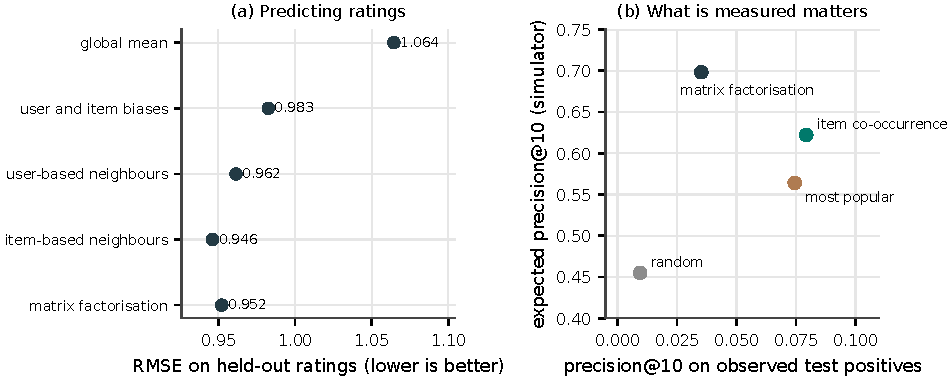
\includegraphics[width=\textwidth]{ch07/recsys_eval}
\caption{(a) Error of five rating predictors on held-out ratings. (b) Precision@10 of four recommenders measured on the observed test positives and, with the
simulator's latent ratings, as the expected share of recommended items that the users would like.}
\label{fig:receval}
\end{figure}

The random split of this experiment measures how well the held-out ratings of known users are
recovered; recommending in the future calls for a split by time, and new users or items need their own protocol.
Offline evaluation has a deeper limitation: it measures how well a recommender predicts what users did when they were shown the
recommendations of the \emph{previous} system. A recommender that suggests something users had never been exposed to cannot get
credit for it offline. The final test is an online experiment (\cref{sec:abtesting}), and because recommendation is a sequence of
decisions with feedback, contextual bandits\index{multi-armed bandit!contextual}\index{multi-armed bandit} (\cref{sec:bandits}) and off-policy\index{off-policy evaluation} evaluation (\cref{lst:ips}) are natural tools.
Recommenders also shape the data they learn from: by showing popular items, they make them more popular, and they can narrow what
each user sees, the \emph{filter bubble}. These feedback loops can increase the homogeneity of what users consume while reducing
the value of the recommendations \citep{chaney2018algorithmic}, which is one more reason to monitor recommenders beyond their
accuracy (\cref{ch:monitoring}).

% =====================================================================
\section{Customer relationship management}\label{sec:crm}

\emph{Customer relationship management\index{customer relationship management (CRM)|textbf}} is the process by which an organisation manages its interactions with its
customers, past, present and potential, using the data it collects about them through every channel: purchases, the
website, the phone, e-mail, social media. Data science turns those data into decisions that improve the relationship
and the business \citep{provost2013data}: whom to target to acquire new customers, what to offer to existing ones
(\emph{cross-selling} and \emph{up-selling}), who is about to leave (\emph{churn}) and is worth retaining, and how much
each customer is worth over the whole relationship (the \emph{customer lifetime value}). Simple summaries of the
behaviour of each customer, such as the \emph{recency}, \emph{frequency} and \emph{monetary} value of their purchases
(RFM), are useful baseline
features in many of these tasks, computed over a stated period before the decision (for acquiring new customers
there may be no history at all).

\subsection{The expected value of a decision}

Most CRM\index{customer relationship management (CRM)} decisions have the same structure: for each customer, decide whether to act (send an offer, call, give a
discount) given a probability estimated by a model and the costs and benefits of each outcome. If contacting a customer
costs $c$, a positive response brings a margin $m$, and the sale would not happen without the contact (so that its
whole margin is due to the contact), contacting them is worth it when the expected value is positive,
\begin{equation}\label{eq:expectedvalue}
  \E[\text{profit}]=p(\text{response}\mid x)\cdot m-c>0
  \quad\Longleftrightarrow\quad
  p(\text{response}\mid x)>\frac{c}{m},
\end{equation}
which is the cost-sensitive\index{cost-sensitive learning} threshold\index{threshold} of \cref{sec:costs} again. If customers may buy anyway, what matters is the increase
caused by the contact: contact when $m\,[P(Y(1)=1\mid x)-P(Y(0)=1\mid x)]>c$, the uplift\index{uplift modelling} of \cref{sec:uplift}. Applying
the rule customer by customer requires calibrated\index{calibration} probabilities (\cref{sec:calibration}): a model that ranks customers
well but overestimates their probabilities will contact too many of them. A profit curve\index{profit curve} computed on labelled
validation data\index{validation set}, as below, uses only the ranking and needs no calibration, but it needs representative data and an
estimate of its uncertainty.

\subsection{Designing a mailing campaign}

Consider a company that sells by catalogue and wants to promote a new product among the customers in its database. Sending
the advertisement to everybody is usually unprofitable. Data science can predict how each customer will respond and use the
predictions to design the campaign\index{mailing campaign} \citep{ling1998data}:
\begin{enumerate}
  \item select a random and sufficiently large sample of customers (a \emph{pilot});
  \item send them the advertisement;
  \item after some time, label each customer of the pilot with 1 if they bought the product and 0 otherwise;
  \item train a probabilistic classifier on the labelled pilot, which estimates the probability that each customer responds;
  \item rank the customers by that probability and draw the \emph{cumulative response curve}, also called the \emph{gains
        chart\index{cumulative gains chart|textbf}}: the share of all the responses obtained as a function of the share of customers contacted;
  \item add the costs and benefits to obtain a \emph{profit curve\index{profit curve|textbf}}, and choose how many customers to contact.
\end{enumerate}
The pilot must be random: only then are its responses a fair sample of how all customers would respond, the same argument
as the hold-out\index{counterfactual hold-out} of \cref{lst:holdout}. Part of the pilot is kept aside to draw the curves, so that the model is not
evaluated on its own training data\index{training set}. The same validation data are then used to choose how many customers to
mail, so the reported maximum is still a development estimate: the chosen model and cutoff should be assessed on
an independent sample, or with a resampling design that repeats the whole selection. The features must describe
the customers before the contact, and the responses must be counted over a completed response window.

\begin{pylisting}[label={lst:crmdata}]{A synthetic customer database and a pilot mailing (file \texttt{crm\_data.py})}
"""A synthetic customer database and a pilot mailing for the CRM examples (Unit 7)."""
import numpy as np

def customers(n=100_000, seed=6):
    rng = np.random.default_rng(seed)
    recency = rng.exponential(120, n)                  # days since the last purchase
    frequency = rng.poisson(3, n)                      # purchases in the last two years
    monetary = rng.gamma(2, 40, n)                     # average order value (EUR)
    age = rng.integers(18, 85, n)
    web = (rng.random(n) < 0.6).astype(int)            # buys online
    logit = (-3.4 - 0.01 * recency + 0.3 * frequency
             + 0.004 * monetary + 0.5 * web - 0.01 * (age - 45))
    X = np.c_[recency, frequency, monetary, age, web]
    # features, true response probability
    return X, 1 / (1 + np.exp(-logit)), rng

def pilot(n_pilot=10_000, seed=6):
    """Mail a random sample; split who responded into training and validation halves."""
    X, p, rng = customers(seed=seed)
    idx = rng.choice(len(p), n_pilot, replace=False)
    y = (rng.random(n_pilot) < p[idx]).astype(int)
    half = n_pilot // 2
    rest = np.setdiff1d(np.arange(len(p)), idx)        # the customers still to be mailed
    return X[idx[:half]], y[:half], X[idx[half:]], y[half:], X[rest], p[rest], rng
\end{pylisting}

\begin{pylisting}[label={lst:mailing}]{Designing a mailing campaign with gains and profit curves}
import numpy as np
from sklearn.ensemble import GradientBoostingClassifier
from sklearn.metrics import roc_auc_score
from crm_data import pilot

X_tr, y_tr, X_val, y_val, X_rest, p_rest, rng = pilot()
print(f"pilot: {len(y_tr) + len(y_val):,} customers mailed, "
      f"response rate {np.r_[y_tr, y_val].mean():.1%}")
model = GradientBoostingClassifier(random_state=0).fit(X_tr, y_tr)
score = model.predict_proba(X_val)[:, 1]
print(f"validation AUC {roc_auc_score(y_val, score):.3f}")
ranked = y_val[np.argsort(-score)]                     # responses in mailing order
gains = np.cumsum(ranked) / ranked.sum()               # share of all responses captured
for f in (0.1, 0.2, 0.5):
    n = int(f * len(ranked))
    print(f"mailing the top {f:.0%}: {gains[n - 1]:.0%} of the responses, "
          f"lift {gains[n - 1] / f:.1f}")

# the campaign: the rest of the base
N = len(p_rest)
share = np.arange(1, len(ranked) + 1) / len(ranked)
CONFIGS = {"config 1": (10_000, 1.50, 30.0), "config 2": (20_000, 0.80, 25.0)}
curves = {}
order_rest = np.argsort(-model.predict_proba(X_rest)[:, 1])   # the real campaign
for name, (fixed, per_mail, margin) in CONFIGS.items():
    mailed = margin * np.cumsum(ranked) * N / len(ranked) - per_mail * share * N - fixed
    profit = np.r_[0.0, mailed]                        # index 0: do not launch at all
    curves[name] = profit
    best = int(np.argmax(profit))
    if best == 0:
        print(f"{name}: do not launch the campaign")
        continue
    n_mail = int(best / len(ranked) * N)
    real = margin * p_rest[order_rest[:n_mail]].sum() - per_mail * n_mail - fixed
    print(f"{name}: mail the top {best / len(ranked):.0%} ({n_mail:,} customers), "
          f"{profit[best]:,.0f} EUR on validation")
    print(f"          true expected profit in the simulation {real:,.0f} EUR; "
          f"mailing everyone {profit[-1]:,.0f} EUR")
\end{pylisting}
\begin{pyoutput}
pilot: 10,000 customers mailed, response rate 6.9%
validation AUC 0.740
mailing the top 10%: 29% of the responses, lift 2.9
mailing the top 20%: 44% of the responses, lift 2.2
mailing the top 50%: 82% of the responses, lift 1.6
config 1: mail the top 55% (49,860 customers), 78,290 EUR on validation
          true expected profit in the simulation 75,243 EUR; mailing everyone 42,380 EUR
config 2: mail the top 70% (62,909 customers), 76,372 EUR on validation
          true expected profit in the simulation 75,715 EUR; mailing everyone 64,150 EUR
\end{pyoutput}

\Cref{lst:crmdata} creates a database of 100,000 customers whose probability of buying depends on their recency, frequency,
monetary value, age and channel. In \cref{lst:mailing}, a pilot of 10,000 customers responds at a rate of 6.9\%. A gradient
boosting\index{gradient boosting}\index{boosting} model trained on half of the pilot has an AUC\index{area under the ROC curve (AUC)} of 0.740 on the other half; the AUC measures its ranking and says nothing about the calibration of its
probabilities. Its gains are substantial
(\cref{fig:campaign}a): mailing the 10\% of customers with the highest scores captures 29\% of all the responses, a
\emph{lift\index{lift|textbf}} of 2.9 over mailing at random, and mailing the top half captures 82\% of them.

The profit curve depends on the costs. The listing compares two configurations:
\begin{itemize}
  \item configuration 1: an initial cost of 10,000~EUR, 1.50~EUR per brochure and a margin of 30~EUR per sale;
  \item configuration 2: an initial cost of 20,000~EUR, 0.80~EUR per brochure and a margin of 25~EUR per sale.
\end{itemize}
With the first, the best decision is to mail the top 55\% of the remaining 90,000 customers, for an estimated profit of
78,290~EUR, while mailing everyone would earn only 42,380~EUR, also estimated on the validation data. With the second, cheaper per brochure, it pays to mail more
customers, the top 70\%, for an estimated 76,372~EUR (\cref{fig:campaign}b). The estimates, computed from 5,000 validation
customers and scaled to the whole database, are close to the simulation's true expected profits of the selected
campaigns (75,243 and 75,715~EUR), which a real company would not know; the cost of the pilot comes on top. The
curves also include not launching at all, with a profit of 0 while the fixed cost can still be avoided: when every
campaign loses money, the best decision is to mail nobody. If the fixed cost has already been paid, it is sunk: it is the
same for every option, so it should be left out of the comparison, and mailing nobody then has an incremental profit of 0. The two configurations end up with similar profits but very different campaigns, which is why the costs must be part of the design from the start.

\begin{figure}[htbp]
\centering
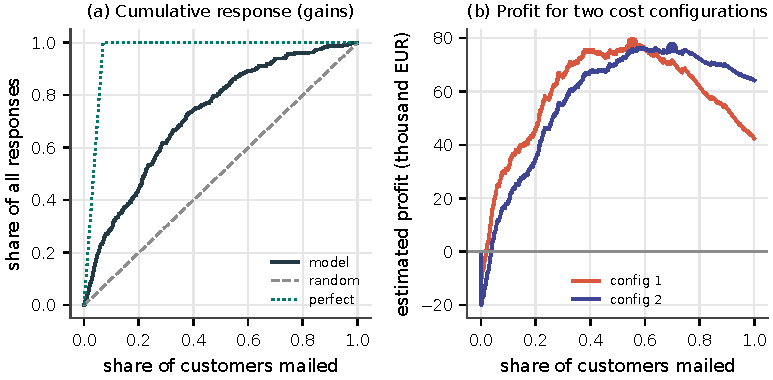
\includegraphics[width=\textwidth]{ch07/campaign}
\caption{(a) Cumulative response curve of the response model, with random and perfect targeting. (b) Profit estimated on the
validation data as a function of the share of customers mailed, for two cost configurations; the point at 0 is
not launching, and the dots mark the decisions selected on the same data.}
\label{fig:campaign}
\end{figure}

\subsection{Uplift modelling}\label{sec:uplift}

The campaign\index{mailing campaign} above targets the customers most likely to buy \emph{after receiving the brochure}. But some of them would
have bought anyway, and the brochure was wasted on them. What matters is the effect of the contact, the difference between
the probability of buying if contacted and if not contacted, which is a causal quantity: the conditional average treatment effect
$\mathrm{CATE}(x)=\E[Y_1-Y_0\mid X=x]$ of the contact (\cref{sec:potentialoutcomes}). Customers
fall into four groups \citep{radcliffe2011real}:
\begin{itemize}
  \item \emph{persuadables\index{uplift modelling!persuadables and sleeping dogs|textbf}}, who buy only if contacted: the only group in which the campaign creates sales (whether they pay for the contact
        is another question);
  \item \emph{sure things}, who buy whether contacted or not: contacting them wastes money;
  \item \emph{lost causes}, who do not buy either way;
  \item \emph{sleeping dogs}, who buy less if contacted, for instance because the contact reminds them to cancel a
        subscription or annoys them: contacting them destroys value.
\end{itemize}
These types are defined by the two potential outcomes of the same customer (\cref{sec:causality}), and only one of
them is ever observed, so the type of an individual cannot be identified. For instance, a population made of half sure things
and half lost causes and another made of half persuadables and half sleeping dogs have the same average effect:
zero. What data can reveal are segments of customers with positive or negative average effects.
A response model ranks sure things and persuadables at the top, and sleeping dogs too if they buy often. \emph{Uplift\index{uplift modelling|textbf}
modelling} estimates the effect instead,
\begin{equation}
  \tau(x)=\E\bigl[Y(1)-Y(0)\mid X=x\bigr],
\end{equation}
the conditional average treatment effect of the contact. In a randomised campaign, it equals the
difference between the response rates of contacted and non-contacted customers with features $x$. This is why uplift modelling needs data from a randomised campaign, in which a random control
group was not contacted, as in an A/B test\index{A/B testing} (\cref{sec:abtesting}). The simplest method trains two models, one on the
contacted customers and one on the control group, and subtracts their predictions; other methods transform the target so
that a single model can be used \citep{jaskowski2012uplift}, or build trees that split directly on differences in uplift
\citep{radcliffe2011real,gutierrez2017causal}. Because the effect of the contact on an individual customer is never observed,
uplift models are evaluated with \emph{uplift} or \emph{Qini curves}, which compare the response rates of the treated and
control customers among those ranked highest \citep{radcliffe2007using}.

\begin{pylisting}[label={lst:uplift}]{A response model against an uplift model on a randomised campaign}
import numpy as np
from sklearn.ensemble import GradientBoostingClassifier

rng = np.random.default_rng(7)
n = 40_000
age, freq, web = rng.integers(18, 85, n), rng.poisson(3, n), rng.random(n) < 0.6
p0 = 1 / (1 + np.exp(-(-3.5 + 0.45 * freq + 0.3 * web)))      # buys without contact
positive_seg = (age < 35) & (freq <= 2)          # contact raises the purchase rate
negative_seg = (age >= 60) & (freq >= 5)          # contact lowers it
# the effect of the contact on the probability of buying
tau = np.where(positive_seg, 0.08, np.where(negative_seg, -0.06, 0.005))
X = np.c_[age, freq, web]
T = rng.random(n) < 0.5                                         # a randomised campaign
y = (rng.random(n) < np.clip(p0 + T * tau, 0, 1)).astype(int)
train, test = np.arange(n) < n // 2, np.arange(n) >= n // 2

gb = lambda: GradientBoostingClassifier(random_state=0)
# classic: who buys if mailed
response = gb().fit(X[train & T], y[train & T])
m1, m0 = gb().fit(X[train & T], y[train & T]), gb().fit(X[train & ~T], y[train & ~T])
scores = {"random": rng.random(n), "response model": response.predict_proba(X)[:, 1],
          "uplift (two models)": m1.predict_proba(X)[:, 1] - m0.predict_proba(X)[:, 1]}
idx = np.flatnonzero(test)
print("top 20% by             true effect   estimated [95% CI]      + segment  - segment")
for name, s in scores.items():
    top = idx[np.argsort(-s[idx])[: len(idx) // 5]]            # the targeted customers
    treated, control = top[T[top]], top[~T[top]]               # randomised, so comparable
    effect = y[treated].mean() - y[control].mean()
    se = np.sqrt(y[treated].var(ddof=1) / len(treated)
                 + y[control].var(ddof=1) / len(control))
    lo, hi = 1000 * (effect - 1.96 * se), 1000 * (effect + 1.96 * se)
    print(f"{name:22s} {1000 * tau[top].mean():+7.1f}   {1000 * effect:+7.1f} "
          f"[{lo:+6.1f}, {hi:+6.1f}]      {positive_seg[top].mean():4.0%}      "
          f"{negative_seg[top].mean():4.0%}")
\end{pylisting}
\begin{pyoutput}
top 20% by             true effect   estimated [95% CI]      + segment  - segment
random                    +8.2     +13.9 [  -8.1,  +35.9]       11%        7%
response model            -9.2     -12.5 [ -41.1,  +16.0]        1%       23%
uplift (two models)      +32.8     +43.8 [ +21.0,  +66.5]       38%        1%
\end{pyoutput}

\Cref{lst:uplift} simulates a randomised campaign of 40,000 customers. The contact raises the probability of buying
by 0.08 in an observable segment of young, infrequent buyers, lowers it by 0.06 in a segment of older, very frequent
buyers, and changes it by 0.005 for everybody else; these segments, not individual persuadables or sleeping dogs, are
what the simulation defines. Contacting a random 20\% of the test customers produces 8.2 extra sales per 1000 contacts
(the true expected effect in the simulation). A response model, which ranks the customers who are most likely to buy
when contacted, does worse than random: it \emph{loses} 9.2 sales per 1000 contacts, because 23\% of the customers it
selects belong to the negative-effect segment (frequent buyers, likely to buy anyway) and only 1\% to the positive one.
The uplift model creates 32.8 extra sales per 1000 contacts, four times as many as random targeting, with 38\% of its
targets in the positive-effect segment and 1\% in the negative one (\cref{fig:uplift}). A real campaign does not know
these true effects, but its randomised design allows them to be \emph{estimated}. Comparing the contacted and the
control customers among those selected by each ranking gives +13.9, $-12.5$ and +43.8 extra sales per 1000 contacts. Their 95\% confidence intervals\index{confidence interval} go from $-8.1$ to +35.9, from $-41.1$ to +16.0 and from +21.0 to +66.5, so only the effect of
the uplift model is clearly positive. Whether it pays is another question: with a margin of 30~EUR and 1.50~EUR per
brochure, 32.8 extra sales per 1000 contacts bring $30\cdot0.0328-1.50\approx-0.52$~EUR per contact. At a 20\% contact
rate, even uplift targeting has a negative expected profit at these prices, and the right decision would be not to launch, or to contact fewer customers
with a larger effect: customers should be ranked by their expected incremental profit, $m\,\tau(x)-c$.

\begin{figure}[htbp]
\centering
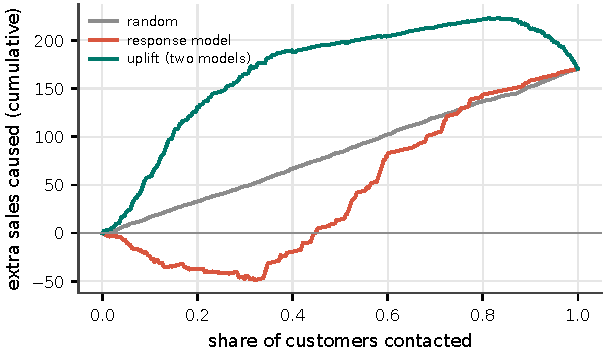
\includegraphics[width=0.72\textwidth]{ch07/uplift}
\caption{Extra sales caused by contacting the customers ranked highest by each score (the true effects of the simulation),
as a function of the share of customers contacted.}
\label{fig:uplift}
\end{figure}

\begin{keyidea}
To decide whom to act on, model the \emph{effect} of the action. Predicting who will buy, churn or recover
answers a different question from predicting whom the offer, the retention call or the treatment will change, and the action creates value only for the customers it changes.
\end{keyidea}

\subsection{Churn and customer lifetime value\extsec}\label{sec:churn}

Customers who leave take their future purchases with them. Predicting \emph{churn\index{churn|textbf}},
which customers are about to leave, is a common CRM\index{customer relationship management (CRM)} task,
and \citet{provost2013data} use it as a running example. A churn model is built like the response model
of the campaign, with three differences:
\begin{itemize}
\item \emph{time}: the features describe each customer at a reference date, from the data of an
\emph{observation window} before it, and the target says whether the customer left during a
\emph{prediction window} after it (for instance, the next three months). Features recorded after the
reference date, such as a request to cancel, leak the answer (\cref{sec:protocols}), and the model must
be evaluated on reference dates later than those used to train it;
\item \emph{value}: losing a customer who spends little costs less than losing one who spends a lot.
The \emph{customer lifetime value\index{customer lifetime value|textbf}} (CLV) estimates the margin that
a customer will bring over the rest of the relationship; with a yearly margin $m$, a probability $r$ of
staying each year and a discount rate $d$, over $T$ years,
\begin{equation}\label{eq:clv}
\mathrm{CLV}=\sum_{t=1}^{T}\frac{m\,r^t}{(1+d)^t},
\end{equation}
and the expected loss from a customer is their probability of leaving times their value;
\item \emph{the action}: a retention offer is a contact like the brochure of the campaign, so the
reasoning of \cref{sec:uplift} applies. The offer creates value only for the customers it keeps, and it
can wake sleeping dogs\index{uplift modelling!persuadables and sleeping dogs}, customers who had not
thought of leaving until the offer reminded them of their contract. A retention campaign therefore needs
a randomised control group, and it should rank customers by the value that the offer saves,
$\tau(x)\,\mathrm{CLV}(x)-c$, where $\tau(x)$ is the reduction in the probability of leaving caused by
the offer and $c$ its cost.
\end{itemize}

% =====================================================================
\section{Interactive applications with Shiny}\label{sec:shinyapps}

A model is only useful if the people who must act on it can use it. A marketing manager will not run a Python script to
decide how many brochures to send, but will happily move a slider in a web page and watch the profit curve\index{profit curve} change.
\emph{Shiny\index{Shiny|textbf}} builds such interactive web applications from code alone \citep{shiny2012,wickham2021mastering}. It was born in the
R community, where RStudio (now Posit) released it as open source in 2012, and Posit also maintains Shiny for Python
\citep{shinypython2024}, which we use here (\cref{tab:shiny}). It communicates with the browser through WebSockets, is built on
a \emph{reactive\index{reactive programming|textbf} programming} model, and can be extended with custom inputs and outputs. We introduced it in
\cref{sec:webapps}; here we look at how it works.

\subsection{The parts of an application}

A Shiny\index{Shiny} application has three components: a \emph{user interface} object, which defines the layout and appearance of the
application; a \emph{server function}, which contains the instructions to build its outputs; and a call that creates the
application from the pair, \texttt{App(app\_ui, server)}. The three usually live in a single file, \texttt{app.py}, which is
launched with \texttt{shiny run app.py}; adding \texttt{-{}-reload} restarts the application whenever the code is saved, which is
convenient while developing it. Shiny for Python also offers \emph{Shiny Express}, a more concise syntax in which the interface and
the outputs are written together, in the order in which they appear on the page.

The user interface is built by nesting functions. \emph{Layout} functions organise the page: a fluid page adapts to the size
of the browser window, and a sidebar layout places the controls in a side panel and the results in a main panel. Static
content (titles, paragraphs, images) is added with functions that mirror the HTML tags. \emph{Control widgets} (sliders, select
boxes, check boxes, numeric and text inputs, date ranges, file uploads, buttons) collect values from the user; the first
two arguments of every widget are an identifier, used to read its value in the server, and a label shown to the user.
\emph{Outputs} (texts, tables, plots, images, HTML) are reserved in the interface with an output function and an identifier,
and built in the server by the matching \emph{render} function, in two steps: add the output to the interface, and tell the
server how to build it.

\subsection{Reactivity}\label{sec:reactivity}

The server never says \emph{when} to recompute an output. An output becomes \emph{reactive\index{reactive programming|textbf}} as soon as the code that builds
it reads the value of an input: Shiny\index{Shiny} records the dependency and, whenever that input changes, re-runs the code and sends the
new output to the browser. The dependencies form a \emph{reactive graph} (\cref{fig:reactivegraph}).

Re-running too much makes applications slow. If an output reads a data set from a remote service and then plots it on a
logarithmic scale chosen with a check box, ticking the box downloads the data again, although only the scale changed. The
solution is a \emph{reactive expression}: a piece of code that reads some inputs and returns a value, created with
the \texttt{@reactive.calc} decorator. Reactive expressions \emph{cache} their value:
the first call computes and stores it, later calls return the stored value, and only when one of the inputs it read changes is
the value marked as obsolete and recomputed at the next call. Expensive steps (loading data, training a model) go in reactive
expressions that depend only on the inputs that affect them, and the outputs call those expressions.

\begin{figure}[htbp]
\centering
\begin{tikzpicture}[font=\scriptsize\sffamily,
  inp/.style={draw=edmteal,fill=edmteal!12,rounded corners=2pt,minimum height=6.5mm,minimum width=24mm,align=center},
  calc/.style={draw=edmgold,fill=edmgold!25,rounded corners=2pt,minimum height=9mm,minimum width=30mm,align=center},
  outp/.style={draw=edmnavy,fill=edmnavy!8,rounded corners=2pt,minimum height=6.5mm,minimum width=27mm,align=center},
  arr/.style={-{Stealth[length=1.5mm]},edmnavy!80}]
  \node[inp] (m) at (0,1.6) {\texttt{model}};
  \node[inp] (f) at (0,0.6) {\texttt{fixed}};
  \node[inp] (c) at (0,-0.4) {\texttt{per\_mail}};
  \node[inp] (g) at (0,-1.4) {\texttt{margin}};
  \node[calc] (r) at (3.9,1.6) {\texttt{ranked()}\\trains and scores (cached)};
  \node[outp] (o1) at (8.2,1.6) {response curve};
  \node[outp] (o2) at (8.2,0.3) {profit curve};
  \node[outp] (o3) at (8.2,-0.9) {summary text};
  \draw[arr] (m) -- (r);
  \draw[arr] (r) -- (o1);
  \draw[arr] (r) -- (o2);
  \draw[arr] (r) -- (o3);
  \foreach \x in {f,c,g} { \draw[arr] (\x.east) -- (o2.west); \draw[arr] (\x.east) -- (o3.west); }
  \node[font=\tiny\sffamily,text=edmteal] at (0,2.25) {inputs};
  \node[font=\tiny\sffamily,text=edmbronze] at (3.9,2.35) {reactive expression};
  \node[font=\tiny\sffamily,text=edmnavy] at (8.2,2.25) {outputs};
\end{tikzpicture}
\caption{The reactive graph of the campaign planner: changing a cost re-runs only the profit curve and the summary; changing
the model retrains it once and updates every output. Each session has its own \texttt{ranked()} and cache.}
\label{fig:reactivegraph}
\end{figure}

Where code is placed also determines how often it runs:
\begin{itemize}
  \item code at the top level of the module, outside the server function (importing libraries, reading data sets, loading
        models), runs once per Python process, when the
        application starts, and is shared by the sessions that the process serves (with several workers or
        replicas, each process loads its own copy);
  \item code inside the server function but outside any render function runs \emph{once per user session}: the place for objects
        that each user needs their own copy of;
  \item code inside a render function runs \emph{every time} an input it reads changes, possibly many times a second while a user
        drags a slider, so it should contain only what must be recomputed to build that output.
\end{itemize}
\Cref{lst:placementapp} marks the three places in a small application, and \cref{lst:placement} measures them by connecting two
users to it: the top-level code runs once, the server function once per user, and the render function every time the slider
moves.

\begin{pylisting}[label={lst:placementapp}]{Three places for code in a Shiny for Python application (file \texttt{placement\_app.py})}
from shiny import App, render, ui

RUNS = {"top level": 0, "server": 0, "render": 0}        # how often each part runs

RUNS["top level"] += 1             # runs once, when the application starts:
CATALOGUE = list(range(1, 1001))   # load data, models and libraries here

app_ui = ui.page_fluid(ui.input_slider("n", "Products", 1, 1000, 10),
                       ui.output_text("total"))

def server(input, output, session):
    RUNS["server"] += 1            # runs once per user session:
    basket = []                    # objects that each user needs their own copy of

    @render.text
    def total():
        RUNS["render"] += 1        # runs every time an input it reads changes
        return f"Total of the first {input.n()} products: {sum(CATALOGUE[:input.n()])}"

app = App(app_ui, server)
\end{pylisting}

\begin{pylisting}[label={lst:placement}]{How often each part runs, measured with two simulated users}
from concurrent.futures import ThreadPoolExecutor
import json
from starlette.testclient import TestClient
import placement_app as pa

_POOL = ThreadPoolExecutor(max_workers=1)

def read_output(ws, name="total", seconds=30, max_messages=50):
    """Read server messages until the value of an output arrives. The blocking read runs
    in a worker thread, so the time limit works on any platform and in any thread."""
    for _ in range(max_messages):
        message = json.loads(_POOL.submit(ws.receive_text).result(timeout=seconds))
        if name in message.get("values", {}):
            return message["values"][name]
    raise RuntimeError(f"output {name} never arrived")


def start(ws, n=10):
    ws.send_text(json.dumps({"method": "init", "data": {
        "n": n, ".clientdata_output_total_hidden": False}}))
    return read_output(ws)

with TestClient(pa.app) as client:
    print(f"application started:                  {pa.RUNS}")
    with client.websocket_connect("/websocket/") as user1:
        start(user1)
        print(f"user 1 opens the page:                {pa.RUNS}")
        for n in (50, 200, 1000):                 # user 1 drags the slider
            user1.send_text(json.dumps({"method": "update", "data": {"n": n}}))
            answer = read_output(user1)
        print(f"user 1 moves the slider three times:  {pa.RUNS}")
        with client.websocket_connect("/websocket/") as user2:
            start(user2)
            print(f"user 2 opens the page:                {pa.RUNS}")
print(f"user 1 sees: {answer}")
\end{pylisting}
\begin{pyoutput}
application started:                  {'top level': 1, 'server': 0, 'render': 0}
user 1 opens the page:                {'top level': 1, 'server': 1, 'render': 1}
user 1 moves the slider three times:  {'top level': 1, 'server': 1, 'render': 4}
user 2 opens the page:                {'top level': 1, 'server': 2, 'render': 5}
user 1 sees: Total of the first 1000 products: 500500
\end{pyoutput}

\subsection{The campaign planner}

\Cref{lst:crmapp} turns the mailing\index{mailing campaign} campaign of \cref{sec:crm} into an application, including the model selector that is a
classic exercise: the user chooses a model (a decision tree\index{decision tree}, a random forest\index{random forest} or nearest neighbours\index{k-nearest neighbours@$k$-nearest neighbours}) and the three costs, and sees
the cumulative response curve, the profit curve\index{profit curve} and a sentence with the best decision. The data are loaded once, outside the server.
Training and scoring happen in the reactive\index{reactive programming} expression \texttt{ranked()}, which depends only on the chosen model, so moving a cost
slider redraws the profit curve and updates the sentence without retraining anything. Each session has its own
\texttt{ranked()}, which caches (stores) the current result until the model changes. This has two limitations. Returning to a model chosen before trains it
again; a cache keyed by the model and the version of the data would avoid this. And training inside the reactive
expression blocks the process while it runs. When training is slow, pretrain the models, or send the work to an
executor (a separate process for CPU-bound Python code) or to a training service, coordinated by an \texttt{ExtendedTask}. An \texttt{ExtendedTask} on its own does not move CPU-bound work off the thread that runs the event loop \citep{shinypython2024}. Rapid movements of a slider may
also be grouped into fewer updates, and the global log of trainings is instrumentation for this demonstration, not an
audit log. The sentence also considers not launching the campaign at all.

\begin{pylisting}[label={lst:crmapp}]{The campaign planner, with a cached reactive expression (file \texttt{crm\_app.py}; run it with \texttt{shiny run crm\_app.py})}
import matplotlib.pyplot as plt
import numpy as np
from shiny import App, reactive, render, ui
from sklearn.ensemble import RandomForestClassifier
from sklearn.neighbors import KNeighborsClassifier
from sklearn.pipeline import make_pipeline
from sklearn.preprocessing import StandardScaler
from sklearn.tree import DecisionTreeClassifier
from crm_data import pilot

X_train, y_train, X_val, y_val, X_rest, _, _ = pilot()   # loaded once per Python process
N = len(X_rest)                                          # customers in the campaign
MODELS = {"Decision tree": lambda: DecisionTreeClassifier(max_depth=5, random_state=0),
          "Random forest": lambda: RandomForestClassifier(200, min_samples_leaf=20,
                                                          random_state=0),
          "Nearest neighbours": lambda: make_pipeline(StandardScaler(),
                                                     KNeighborsClassifier(100))}
TRAININGS = []                                           # a log, to see the caching

def profit_curve(ranked, fixed, per_mail, margin, n=N):
    """Profit of not launching (index 0) and of mailing the top k customers, for every k,
    scaled to n customers; the fixed cost is paid only if the campaign is launched."""
    ranked = np.asarray(ranked)
    share = np.arange(1, len(ranked) + 1) / len(ranked)
    mailed = margin * np.cumsum(ranked) * n / len(ranked) - per_mail * share * n - fixed
    return np.r_[0.0, mailed]

def decision(profit, n_validation):
    """The best action: not launching (index 0) or mailing the top customers."""
    best = int(np.argmax(profit))
    if best == 0:
        return "Do not launch the campaign: every mailing loses money"
    return (f"Mail the top {best / n_validation:.0%} of {N:,} customers: "
            f"profit {profit[best]:,.0f} EUR")

app_ui = ui.page_sidebar(
    ui.sidebar(
        ui.input_select("model", "Model", list(MODELS)),
        ui.input_slider("fixed", "Initial cost (EUR)", 0, 40_000, 10_000, step=1_000),
        ui.input_slider("per_mail", "Cost per brochure (EUR)", 0.1, 3.0, 1.5, step=0.1),
        ui.input_slider("margin", "Profit per sale (EUR)", 5, 60, 30),
    ),
    ui.output_text("summary"),
    ui.layout_columns(ui.output_plot("response"), ui.output_plot("profit_plot")),
    title="Mailing campaign planner",
)

def server(input, output, session):
    @reactive.calc                     # cached: recomputed only when the model changes
    def ranked():
        TRAININGS.append(input.model())
        model = MODELS[input.model()]().fit(X_train, y_train)
        return y_val[np.argsort(-model.predict_proba(X_val)[:, 1])]

    def profit():
        return profit_curve(ranked(), input.fixed(), input.per_mail(), input.margin())

    @render.text
    def summary():
        return decision(profit(), len(ranked()))

    @render.plot
    def response():
        r = ranked()
        x = np.arange(1, len(r) + 1) / len(r)
        fig, ax = plt.subplots()
        ax.plot(x, np.cumsum(r) / r.sum(), label=input.model())
        ax.plot([0, 1], [0, 1], "--", label="random")
        ax.set(xlabel="share of customers mailed", ylabel="share of responses")
        ax.legend()
        return fig

    @render.plot(alt="Profit curve")
    def profit_plot():
        p = profit()
        fig, ax = plt.subplots()
        ax.plot(np.arange(len(p)) / (len(p) - 1), p)        # 0: not launching
        ax.axhline(0, color="grey")
        ax.set(xlabel="share of customers mailed", ylabel="profit (EUR)")
        return fig

app = App(app_ui, server)                                # run: shiny run crm_app.py
\end{pylisting}

The behaviour that matters can be tested automatically, as in \cref{sec:webapps}. \Cref{lst:crmtest} checks the profit
computation, including the decision not to launch, against small cases worked out by hand, checks that the page contains every control and output, and then connects to
the application as a browser would, through its WebSocket protocol. It changes the cost per brochure, checks that the sentence
changes and that the model was \emph{not} retrained (the application keeps a log of its trainings), then changes the model and checks
that it was retrained exactly once. With a decision tree and the costs of the first configuration, the application recommends mailing
the top 71\% of the 90,000 customers, for a profit of 69,515~EUR; at 0.50~EUR per brochure, it recommends 84\%, for 135,368~EUR. These tests
check the arithmetic, the identifiers of the page and the reactive behaviour of the server through its WebSocket
protocol; they do not exercise the rendering in a browser or its JavaScript, which a browser test, for instance
with Playwright, can check, together with both plots. The helper that reads the outputs gives up after 50 messages,
and a time limit stops a regression from blocking the test run forever. The blocking read runs in a worker thread with a
timeout, which works on any operating system and in any thread; an alarm signal would work only on Unix, in the main thread,
and would replace the handler of the whole process. The test client speaks the internal protocol of
Shiny\index{Shiny}, which may change between versions, so the requirements file pins them (here Shiny 1.8.0, Starlette 1.7.0 and
pytest 9.1.1).

\begin{pylisting}[label={lst:crmtest}]{Testing the planner: profit, page, and reactive caching (file \texttt{test\_crm\_app.py}; run it with \texttt{pytest})}
from concurrent.futures import ThreadPoolExecutor
import json

import numpy as np
import pytest
from starlette.testclient import TestClient
import crm_app

@pytest.fixture(scope="module")
def client():
    with TestClient(crm_app.app) as c:
        yield c

_POOL = ThreadPoolExecutor(max_workers=1)

def read_output(ws, name="summary", seconds=30, max_messages=50):
    """Read server messages until the value of an output arrives. The blocking read runs
    in a worker thread, so the time limit works on any platform and in any thread."""
    for _ in range(max_messages):
        message = json.loads(_POOL.submit(ws.receive_text).result(timeout=seconds))
        if name in message.get("values", {}):
            return message["values"][name]
    raise AssertionError(f"output {name} never arrived")


def test_profit_curve():                     # unit tests, computed by hand
    p = crm_app.profit_curve(np.array([1, 0, 1, 0]), fixed=10, per_mail=1, margin=5, n=4)
    assert np.allclose(p, [0, -6, -7, -3, -4])     # index 0: do not launch
    assert crm_app.decision(p, 4).startswith("Do not launch")
    p = crm_app.profit_curve(np.array([1, 0, 1, 0]), fixed=1, per_mail=1, margin=5, n=4)
    assert crm_app.decision(p, 4).startswith("Mail the top 75%")

def test_page_has_the_controls(client):
    page = client.get("/").text
    for name in ("model", "fixed", "per_mail", "margin", "summary", "response",
                 "profit_plot"):
        assert f'id="{name}"' in page

def test_costs_do_not_retrain_but_the_model_does(client):
    crm_app.TRAININGS.clear()
    with client.websocket_connect("/websocket/") as ws:
        ws.send_text(json.dumps({"method": "init", "data": {
            "model": "Decision tree", "fixed": 10_000, "per_mail": 1.5, "margin": 30,
            ".clientdata_output_summary_hidden": False}}))
        first = read_output(ws)
        ws.send_text(json.dumps({"method": "update", "data": {"per_mail": 0.5}}))
        cheaper = read_output(ws)
        assert cheaper != first and crm_app.TRAININGS == ["Decision tree"]
        new_model = {"model": "Nearest neighbours"}
        ws.send_text(json.dumps({"method": "update", "data": new_model}))
        read_output(ws)
        assert crm_app.TRAININGS == ["Decision tree", "Nearest neighbours"]
    print(f"\n  1.50 EUR per brochure: {first}\n  0.50 EUR per brochure: {cheaper}")
\end{pylisting}
\begin{pyoutput}
============================= test session starts ==============================
collecting ... collected 3 items

test_crm_app.py::test_profit_curve PASSED
test_crm_app.py::test_page_has_the_controls PASSED
test_crm_app.py::test_costs_do_not_retrain_but_the_model_does 
  1.50 EUR per brochure: Mail the top 71% of 90,000 customers: profit 69,515 EUR
  0.50 EUR per brochure: Mail the top 84% of 90,000 customers: profit 135,368 EUR
PASSED

============================== 3 passed in 2.76s ===============================
\end{pyoutput}

\subsection{Sharing applications}

There are several ways of sharing a Shiny\index{Shiny} for Python application. The simplest is to share its code, for instance in a Git\index{Git}
repository: users install the packages listed in its requirements file and launch it with \texttt{shiny run}. \emph{Shinylive\index{Shinylive|textbf}}
exports the application to a set of static files that run entirely in the user's browser, with Python compiled to
WebAssembly, so that it can be published on any web server, or even shared as a link, with no Python server behind it; the price is
that the code and the data travel to the browser, and not every package is available. To host the application as a web service that
anyone can open, it can be deployed to \emph{Posit Connect Cloud\index{Posit Connect Cloud|textbf}}, Posit's hosting service, for instance
directly from a Git repository with a requirements file, or to \emph{Posit Connect}, its platform for an organisation's
own infrastructure, which adds authentication, encrypted connections and administration tools. Posit is migrating
its older service, shinyapps.io, to Connect Cloud during 2027 \citep{posit2026connectcloud}, so new applications should
follow the current deployment documentation; or it can be packaged in a container\index{containers} and run like any other web service (\cref{sec:packaging}).

% =====================================================================
% ---------------------------------------------------------------------
\section{The applications across the life cycle}\label{sec:applifecycle}

The two applications of this unit go through every stage of the life cycle described in the
introduction, and each stage uses the tools of an earlier unit. \Cref{tab:applifecycle} follows a
recommender and a customer campaign (a response, uplift or churn model) from evaluation to updating.

\begin{table}[htbp]
\centering\small
\caption{A recommender and a customer campaign through the life cycle of a model.}\label{tab:applifecycle}
\begin{tabularx}{\textwidth}{@{}>{\raggedright\arraybackslash}p{1.6cm}>{\raggedright\arraybackslash}X>{\raggedright\arraybackslash}X@{}}
\toprule
Stage & Recommender & Customer campaign\\
\midrule
Evaluate & ranking metrics on a split by time, with coverage and novelty, against a popularity baseline
(\cref{sec:receval}) & AUC and gains on a held-out part of the pilot; profit curve on validation data,
confirmed on a separate test set (\cref{sec:crm})\\
Decide & how many items to show and where; filters for items already bought, unavailable or not allowed &
whom to contact, by expected incremental profit, $m\,\tau(x)-c$, or by the value that a retention offer
saves (\cref{sec:uplift,sec:churn})\\
Deploy & candidates precomputed in batch and ranked at request time within a latency budget
(\cref{sec:deployoptions}) & batch scoring of the customer base before each campaign, and a planner for
the people who decide (\cref{sec:shinyapps})\\
Monitor & click-through and conversion, coverage, the share of recommendations taken by the most popular
items, drift of the catalogue and of the users (\cref{ch:monitoring}) & response and uplift in a random
control group kept in every campaign, drift of the customer features, calibration of the probabilities\\
Update & frequent retraining as items and users arrive; new versions through A/B tests or interleaving,
and bandits for short-lived content (\cref{sec:abtesting,sec:bandits}) & retraining with the randomised
results of each campaign, so that each campaign also evaluates the current model\\
\bottomrule
\end{tabularx}
\end{table}

Both applications create their own future data. A recommender decides which items users see, so its logs
over-represent what it recommended; a campaign decides whom to contact, so the responses of the customers
it skipped are never observed. In both cases a small share of randomised decisions, logged with their
probabilities (\cref{lst:ips}), keeps the data usable for evaluating the next model, at a cost that can be
estimated in advance, as for the hold-out of \cref{lst:holdout}. In both cases, too, the decision depends on
costs and constraints that change more often than the model: prices, margins, budgets and the items that
cannot be recommended belong in the application, where the people who decide can change them, as in the
planner of \cref{lst:crmapp}.

\section{Summary}\label{sec:summary7}

\begin{itemize}
  \item Recommender systems\index{recommender system} suggest items from interactions (collaborative filtering\index{collaborative filtering}), from item descriptions (content-based\index{content-based filtering}
        filtering) or from both (hybrids).
  \item User-based\index{collaborative filtering!user-based} collaborative filtering predicts ratings as similarity\index{similarity measure}-weighted averages of the ratings of similar users;
        item-based\index{collaborative filtering!item-based} filtering compares items instead, which is more stable and scales better. Similarities computed on few common
        items are unreliable.
  \item Matrix factorisation\index{matrix factorisation} represents users and items by latent factors; it was central to the Netflix\index{Netflix Prize} Prize, whose data also
        showed that anonymised ratings can identify people.
  \item Content-based filtering solves the cold start\index{cold start} of new items and gives explainable\index{explainability} recommendations, but tends to
        overspecialise.
  \item Rating errors evaluate rating prediction, and ranking metrics evaluate recommendation lists; the candidate set, the
        relevance labels and the process that decides what is observed must be stated, because ratings are missing not
        at random. Coverage\index{coverage}, novelty\index{novelty} and diversity\index{diversity!of recommendations} complement accuracy, popularity is a strong baseline, and online
        experiments give the final assessment.
  \item In CRM\index{customer relationship management (CRM)}, decisions follow the expected incremental value of acting, which combines the change that the action causes
        with its costs and benefits; not acting is always one of the options. A mailing\index{mailing campaign} campaign is designed with a random pilot, a probabilistic classifier, a cumulative response curve and a
        profit curve\index{profit curve}, whose optimum depends on the costs.
  \item Uplift\index{uplift modelling} modelling targets the customers whose behaviour the action changes; a response model can do worse than random by
        targeting sure things\index{uplift modelling!persuadables and sleeping dogs} and sleeping dogs.
\item Churn models need features observed before a reference date and a target observed after it, a
temporal evaluation, and a ranking by the value that the retention offer saves; retention offers, like
any contact, can wake sleeping dogs.
  \item Shiny\index{Shiny} builds interactive applications from a user interface and a reactive\index{reactive programming} server; reactive expressions cache expensive
        computations, and the placement of code determines how often it runs.
\item Both applications go through the whole life cycle: offline evaluation, a decision rule with costs,
batch or online deployment, monitoring with a randomised control share, and updates through experiments.
\end{itemize}

\section*{Bibliographic notes}
\phantomsection\addcontentsline{toc}{section}{Bibliographic notes}

\citet{segaran2007programming} is a practical introduction to collaborative filtering\index{collaborative filtering}, and \citet{aggarwal2016recommender} and
\citet{ricci2022recommender} cover recommender systems\index{recommender system} in depth. \citet{koren2009matrix} explain matrix factorisation\index{matrix factorisation} as used in the
Netflix\index{Netflix Prize} Prize, \citet{herlocker2004evaluating} the evaluation of collaborative filtering, and \citet{kaminskas2016diversity} the measures
beyond accuracy. \citet{provost2013data} present the expected value framework, cumulative response and profit curves\index{profit curve} for business
problems, and \citet{gutierrez2017causal} review uplift\index{uplift modelling} modelling. \citet{wickham2021mastering} is a reference on Shiny\index{Shiny} and its reactive\index{reactive programming}
model.

\section*{Exercises}
\phantomsection\addcontentsline{toc}{section}{Exercises}

\begin{enumerate}[label=\textbf{7.\arabic*},ref=7.\arabic*,leftmargin=*,itemsep=6pt]
  \item\label{exr7:euclid} Two users rated three common films (4, 2, 5) and (5, 1, 3). Compute their Euclidean\index{Euclidean distance}-based similarity\index{similarity measure}.
  \item\label{exr7:pearson} Why is the Pearson\index{Pearson correlation} correlation of two users with exactly two films in common always $+1$ or $-1$ when each
        of them rated the two films differently? What can be
        done about it?
  \item\label{exr7:predict} Three users have similarities 0.9, 0.5 and $-0.3$ with you and rated a film 4, 2 and 5. Predict your rating with
        \cref{eq:usercf}.
  \item\label{exr7:scale} An online shop has 10 million customers and 50,000 products. Would you use user-based\index{collaborative filtering!user-based} or item-based\index{collaborative filtering!item-based} collaborative
        filtering\index{collaborative filtering}, and what would you precompute?
  \item\label{exr7:params} How many parameters has a matrix factorisation\index{matrix factorisation} with $k=50$ factors and biases on the Netflix\index{Netflix Prize} Prize data? Compare
        them with the number of ratings.
  \item\label{exr7:metrics} A top-5 list has relevant items in positions 1 and 4, and the user has 3 relevant items in total. Compute
        precision@5, recall@5 and NDCG\index{NDCG}@5.
  \item\label{exr7:cold} How would you recommend items to a user who has just registered? And recommend an item added today?
  \item\label{exr7:tfidf} With the classical formula $\mathrm{idf}(t)=\log(n/\mathrm{df}(t))$, what weight does a term that appears in the
        description of every item receive? How does this differ from the default of scikit-learn's \texttt{TfidfVectorizer}?
  \item\label{exr7:campaign} A company has 100,000 customers, 5\% of whom would buy. The top 20\% of a model's ranking contains half of the
        buyers. With the costs of configuration 1, compare the profit of mailing\index{mailing campaign} the top 20\% with that of mailing everyone.
  \item\label{exr7:threshold} Using \cref{eq:expectedvalue}, compute the probability above which a customer is worth contacting in each
        configuration of \cref{lst:mailing}. How does this explain why the second configuration mails more customers?
  \item\label{exr7:lift} The response rate of the pilot is 6.9\% and the top 10\% has a lift\index{lift} of 2.9. What is the response rate in the top
        10\%?
  \item\label{exr7:groups} For each pair (buys if contacted, buys if not contacted) $\in\{0,1\}^2$, name the group of customers. Which group
        should never be contacted?
  \item\label{exr7:upliftcalc} Among the customers ranked highest by an uplift\index{uplift modelling} model, 1000 were contacted at random and 1000 were kept as a
        control: 80 of the contacted and 50 of the controls bought. Estimate the uplift and the extra sales per 1000 contacts.
  \item\label{exr7:place} In a Shiny\index{Shiny} application, where would you put the code that reads a 2~GB data set, the code that creates each user's
        shopping basket, and the code that filters the data by the dates chosen in a widget?
  \item\label{exr7:graph} In the planner of \cref{lst:crmapp}, which outputs are recomputed when the margin changes, and which when the model
        changes? How many times is a model trained if a user drags the margin slider through 50 values?
  \item\label{exr7:privacy} The Netflix Prize data contained no names. How could users be re-identified, and what does this teach about
        releasing behavioural data?
  \item\label{exr7:integrated} (An integrated case.) Using the randomised campaign of \cref{lst:uplift}, with a margin of
        30~EUR and 1.50~EUR per contact: (a) compare not launching with contacting the top customers of the response model
        and of the uplift model, in expected \emph{incremental} profit; (b) choose the model and the share of customers to
        contact on validation data, and estimate the profit of the chosen policy on a separate test set, with an interval;
        (c) check in the planner of \cref{lst:crmapp} that changing the costs updates the decision without retraining.
\item\label{exr7:clv} A customer brings a margin of 120~EUR a year, stays each year with probability 0.8,
and future margins are discounted at 5\% a year. Compute their lifetime value over the next five years
with \cref{eq:clv}. A retention offer costs 20~EUR and reduces their probability of leaving this year
from 0.30 to 0.20. Is it worth making?
\item\label{exr7:lifecycle} A news site wants to recommend articles on its home page. For each stage of
\cref{tab:applifecycle}, say what changes with respect to a film recommender, given that articles lose
their interest within hours.
\item\label{exr7:modelcard} Write the model card\index{model card} of the uplift model of the mailing
campaign, following \cref{lst:modelcard}: intended use and uses it is not meant for, data and
control group, evaluation (Qini curve and incremental profit on held-out data), results for
relevant groups of customers, limitations, and the monitoring plan of \cref{tab:applifecycle}.
\end{enumerate}

\section*{Solutions}
\phantomsection\addcontentsline{toc}{section}{Solutions}

\begin{description}[font=\bfseries,leftmargin=0pt,itemsep=5pt]
  \item[\ref{exr7:euclid}] $d=\sqrt{1^2+1^2+2^2}=\sqrt6\approx2.45$, so the similarity\index{similarity measure} is $1/(1+2.45)\approx0.29$.
  \item[\ref{exr7:pearson}] Two points always lie exactly on a line, increasing or decreasing, so the correlation is $\pm1$ whatever the
        ratings (or undefined if a user gave both films the same rating). Require a minimum number of common items, or shrink the
        similarity towards 0 by a factor such as $\min(n,50)/50$, where $n$ is the number of common items.
  \item[\ref{exr7:predict}] Only positive similarities are used: $(0.9\cdot4+0.5\cdot2)/(0.9+0.5)=4.6/1.4\approx3.29$.
  \item[\ref{exr7:scale}] Item-based\index{collaborative filtering!item-based}: the item--item similarities (for each product, its few hundred most similar products) are
        precomputed offline and updated, say, daily; at request time, the recommendations combine the similar items of the products in
        the customer's history, which is fast. Comparing each customer with 10 million others at request time would be too slow. A dense $50{,}000\times50{,}000$ matrix
        of 4-byte similarities would take 10~GB; keeping only a few hundred neighbours per product keeps it small.
  \item[\ref{exr7:params}] $(480{,}189+17{,}770)\cdot50\approx24.9$ million factors, plus about 0.5 million biases: some 25 million parameters
        for 100 million ratings, which is why regularisation is needed.
  \item[\ref{exr7:metrics}] Precision@5 $=2/5=0.4$; recall@5 $=2/3\approx0.67$. $\mathrm{DCG}=1/\log_22+1/\log_25=1+0.431=1.431$; the ideal list has the
        three relevant items first, $\mathrm{IDCG}=1+1/\log_23+1/\log_24=2.131$; NDCG\index{NDCG}@5 $=1.431/2.131\approx0.67$.
  \item[\ref{exr7:cold}] New user: recommend popular or highly rated items, possibly by segment (country, device), ask for a few ratings or
        preferences at registration, and switch to personalised recommendations as interactions arrive (or use a bandit\index{multi-armed bandit}). New item: use its
        content (attributes, description) with a content-based\index{content-based filtering} or hybrid model, and give it some exposure to collect interactions. A content-based recommender\index{recommender system} personalises for a user only once some of
        their preferences are known, explicitly or from their first interactions.
  \item[\ref{exr7:tfidf}] The classical IDF is $\log1=0$: a term that every item has does not distinguish any item. The default of
        scikit-learn, $\log\frac{1+n}{1+\mathrm{df}}+1$, gives it an IDF of 1, so it is not removed automatically, although
        frequent terms still weigh less than rare ones.
  \item[\ref{exr7:campaign}] Top 20\%: 20,000 brochures and 2,500 sales: $2{,}500\cdot30-20{,}000\cdot1.5-10{,}000=35{,}000$~EUR, if these sales happen only because of the brochure. Everyone: 5,000
        sales: $150{,}000-150{,}000-10{,}000=-10{,}000$~EUR.
  \item[\ref{exr7:threshold}] $1.50/30=0.05$ and $0.80/25=0.032$. With the second configuration it pays to contact customers with a lower
        probability of responding, who are further down the ranking, so the optimal campaign\index{mailing campaign} is larger. The fixed cost of launching does not change these marginal thresholds: it only decides
        whether the campaign is launched at all.
  \item[\ref{exr7:lift}] $2.9\cdot6.9\%\approx20\%$.
  \item[\ref{exr7:groups}] (1,0) persuadables\index{uplift modelling!persuadables and sleeping dogs}, (1,1) sure things, (0,0) lost causes, (0,1) sleeping dogs, whom contacting can only harm. Individual types are
        never observed, so in practice one avoids segments with a negative average effect.
  \item[\ref{exr7:upliftcalc}] $80/1000-50/1000=0.03$: about 30 extra sales per 1000 contacts. With 1000 treated and 1000 controls, the standard
        error is $\sqrt{0.08\cdot0.92/1000+0.05\cdot0.95/1000}\approx0.011$, so an approximate 95\% interval for the uplift\index{uplift modelling} goes
        from 0.0084 to 0.0516.
  \item[\ref{exr7:place}] Reading the data set: at the top of the application, outside the server, so that it runs once
        per Python process (each worker or replica loads its own copy). The basket: inside the
        server function, outside the render functions, once per session. The filtering by dates: in a reactive\index{reactive programming} expression (or render function)
        that reads the date widget, since it must be recomputed when the dates change.
  \item[\ref{exr7:graph}] The margin affects the profit curve\index{profit curve} and the summary; the model affects all three outputs, through \texttt{ranked()}.
        Dragging the margin through 50 values trains no additional model (one was trained when the session
        opened): the reactive expression returns its cached value.
  \item[\ref{exr7:privacy}] By matching the dates and ratings of a few films with public reviews on other sites: few people rate the same rare
        films on the same days. Behavioural data are often unique to a person even without names, so removing identifiers does not anonymise
        them (\cref{sec:fairness}).
  \item[\ref{exr7:integrated}] (a) Only the uplift model targets incremental sales: at these prices its top 20\% brings
        $30\cdot0.0328-1.50\approx-0.52$~EUR per contact, so the best options are not launching or contacting a smaller group
        with a larger effect; the response model loses money. (b) Split the data into training, validation and test parts, and choose the model and the
        share of customers on validation. On the test part, estimate the value of the chosen policy: among the selected
        customers, the difference between treated and control customers in margin minus contact costs, per contact; its
        interval resamples customers within the treated and the control groups (or uses the normal approximation for the
        two proportions). It is honest because the test data took no part in the choice. (c) \Cref{lst:crmtest} does exactly this for one change of costs.
\item[\ref{exr7:clv}] $\mathrm{CLV}=\sum_{t=1}^{5}120\cdot0.8^t/1.05^t\approx285.41$~EUR. The offer reduces
the probability of losing that value by 0.10, so it saves $0.10\cdot285.41\approx28.54$~EUR on average for
a cost of 20~EUR: about 8.54~EUR per customer, if the reduction is a causal effect measured with a
control group (\cref{sec:uplift}).
\item[\ref{exr7:lifecycle}] Evaluate: split by hour, and measure on the clicks of the following hours;
nearly every article is new, so cold start\index{cold start} is the rule and content-based or hybrid
models are needed. Decide: positions and the diversity of topics on the page. Deploy: features and
candidates updated continuously. Monitor: click-through by hour, the share of fresh articles, and the
topics of the news. Update: retraining every few hours or online learning, and bandits for headlines
and articles that live for hours (\cref{sec:bandits}).
\item[\ref{exr7:modelcard}] Intended use: choosing whom to send the brochure, within a budget; not
for other products or for deciding prices. Data: the pilot, with the randomised control group that
makes uplift measurable. Evaluation: the Qini curve and the incremental profit at the chosen cut-off,
with intervals from a bootstrap over customers. Groups: uplift by segment, to check that the model
does not concentrate the offers on one region or age group without reason. Limitations: one past
campaign, effects that may change with the season or the offer, and sleeping dogs that are hard to
estimate with few responses. Monitoring: response and uplift in a random control group kept in
every campaign, and drift of the customer features.
\end{description}

